% Basic drawings
% https://www.sharelatex.com/blog/2013/08/27/tikz-series-pt1.html
% https://www.tug.org/TUGboat/tb29-1/tb91walczak.pdf
\documentclass[border=1pt,tikz]{standalone}
\usepackage{tikz}

\begin{document}


% SET: critical region
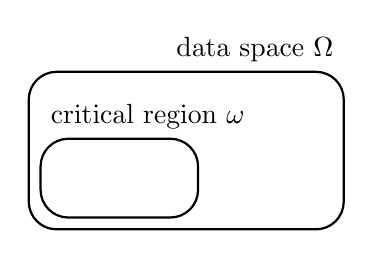
\begin{tikzpicture}[scale=1.0]
  \draw[black,rounded corners=10,thick]
     (0,0) rectangle (4,2)
     node[above left] {data space $\Omega$};
  \draw[black,rounded corners=10,thick,shift={(0.15,0.15)}]
    (2,0) rectangle (0,1)
     node[above right] {critical region $\omega$};
\end{tikzpicture}



% SET: overlapping critical regions
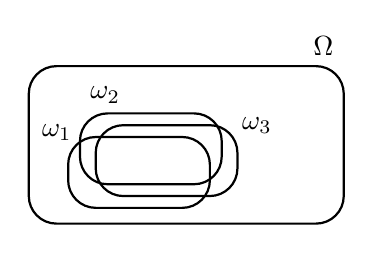
\begin{tikzpicture}[scale=1.0]
  \draw[black,rounded corners=10,thick]
     (0,0) rectangle (4,2)
     node[above left] {$\Omega$};
  \begin{scope}[shift={(0.35,0.05)}]
    \draw[black,rounded corners=10,thick,shift={(0.15,0.15)},scale=0.90]
      (2,0) rectangle (0,1)
       node[above left=-5pt] {$\omega_1$};
    \draw[black,rounded corners=10,thick,shift={(0.30,0.45)},scale=0.90]
      (2,0) rectangle (0,1)
       node[right=0pt,above right] {$\omega_2$};
    \draw[black,rounded corners=10,thick,shift={(0.50,0.30)},scale=0.90]
      (0,0) rectangle (2,1)
       node[right=-2pt] {$\omega_3$};
  \end{scope}
\end{tikzpicture}


\end{document}